% This work by Jeremy A. Hansen is licensed under a Creative Commons 
% Attribution-NonCommercial-ShareAlike 3.0 Unported License, 
% as described at http://creativecommons.org/licenses/by-nc-sa/3.0/legalcode

Pointers do just what they sound like they do. 
They point to a space in memory, usually a location occupied by a variable. 
A pointer is an address in memory. 
The pointer itself is a variable, but it also refers to a variable. 
It is declared using an asterisk following the data type:

\noindent\begin{minipage}{\linewidth}\begin{lstlisting}
int *ptr; 
\end{lstlisting}\end{minipage}

The variable named \Code{ptr} is of type \Code{int*}, an ``integer pointer'' that stores the address of a variable of type \Code{int}.

To indicate that a pointer variable is not pointing toward any usable data, we often set its value to \Code{NULL}, which is defined as zero when you \Code{\#include <cstdlib>}:

\noindent\begin{minipage}{\linewidth}\begin{lstlisting}
int *ptr = NULL;
\end{lstlisting}\end{minipage}

C++11 provides a dedicated null pointer object called \Code{nullptr} that can be used similarly:

\noindent\begin{minipage}{\linewidth}\begin{lstlisting}
int *ptr = nullptr;
\end{lstlisting}\end{minipage}

There are two operators used in conjunction with pointers. 
The \Code{*} operator, beyond being used for multiplication and for pointer declarations, also acts as the \Keyword{dereference operator}. 
The dereference operator changes the pointer into the value it is pointing to.
It ``follows'' the address stored in the pointer and returns whatever is in that location.

The \Code{\&} operator is the \Keyword{reference operator}. 
The dereference operator returns the memory address of the variable it precedes. 
You will use this to produce a pointer to the indicated variable.

Let's declare pointer \Code{p} and use it:

\noindent\begin{minipage}{\linewidth}\begin{lstlisting}
int *p;       // Declare an int pointer
int var1 = 2; // Declare an int, set it to 2
p = &var1;    // Take the address of var1 and store it in p
cout << *p;   // Go to the address stored in p;
              // return the value; print it out
\end{lstlisting}\end{minipage}

\noindent The output of this code is:

\noindent \Code{2}

Here is a slightly longer example:

\noindent\begin{minipage}{\linewidth}\begin{lstlisting}
int *p;
int var1 = 2;
int var2 = 4;
p = &var1; // Take the address of var1 and store it in p
*p = var2; // Go to the address stored in p; 
           // assign it the value stored in var2

// The preceding two lines equivalent are to var1 = var2
cout << *p << endl;
cout << var1 << endl;
cout << var2 << endl;
\end{lstlisting}\end{minipage}

The output of this code is:

\noindent \Code{4}

\noindent \Code{4}

\noindent \Code{4}

\begin{figure}[tb]
  \centering
  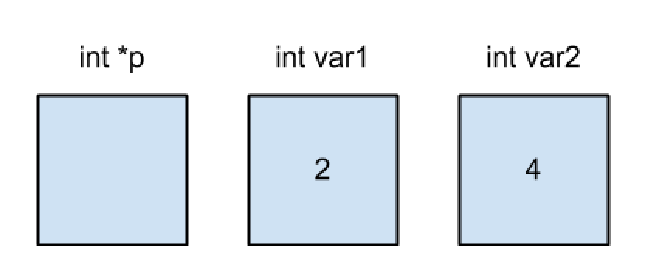
\includegraphics[width=0.6\textwidth]{diagrams/pointer-example-1.pdf}
  \caption{The state of the variables after lines 1-3} \label{fig:pointer-example-1} 
\end{figure}

\begin{figure}[tb]
  \centering
  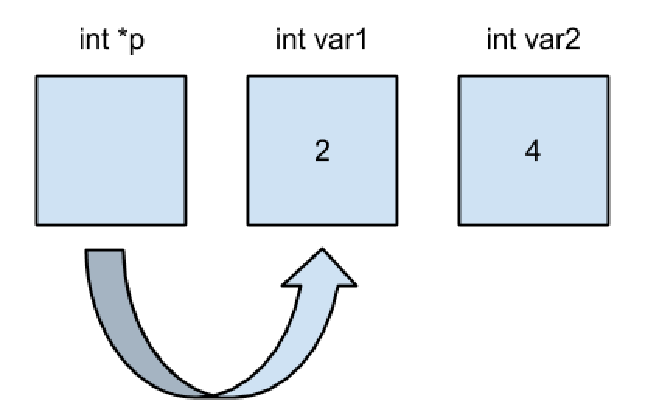
\includegraphics[width=0.6\textwidth]{diagrams/pointer-example-2.pdf}
  \caption{The state of the variables after line 4} \label{fig:pointer-example-2} 
\end{figure}

\begin{figure}[tb]
  \centering
  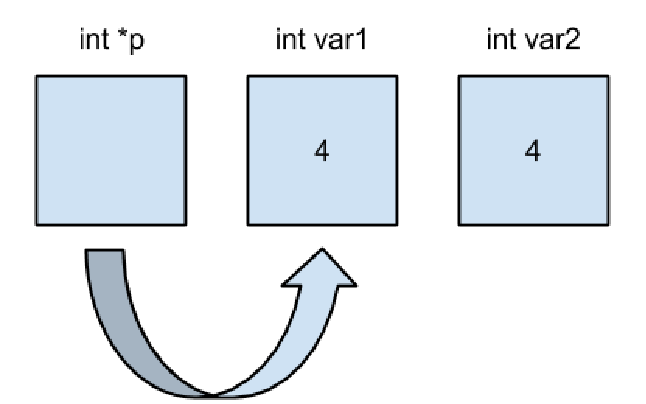
\includegraphics[width=0.6\textwidth]{diagrams/pointer-example-3.pdf}
  \caption{The state of the variables after line 5} \label{fig:pointer-example-3} 
\end{figure}

Figure \ref{fig:pointer-example-1} shows the state of the variables in the second example after they are declared and initialized (lines 1-3).
After the fourth line is executed, \Code{p} will store the address of \Code{var1}. Figure \ref{fig:pointer-example-2} shows the state of the variables.
After the fifth line of code is executed, the location where \Code{p} points is assigned the value stored in \Code{var2}.
Since \Code{p} contains the address of \Code{var1}, \Code{var1} receives that value. Figure \ref{fig:pointer-example-3} shows the state of the variables.

Use caution when declaring pointers.
If you are declaring more than one pointer in a single line, make sure to indicate each pointer variable with the \Code{*} before the variable name.  
Here is a correct declaration of two pointers:

\noindent\begin{minipage}{\linewidth}\begin{lstlisting}
int *p, *q;
\end{lstlisting}\end{minipage}

This results in an integer pointer named \Code{p} and an integer pointer named \Code{q}. 
Contrast that with the below code:

\noindent\begin{minipage}{\linewidth}\begin{lstlisting}
int *p, q;
\end{lstlisting}\end{minipage}

This results in an integer pointer named \Code{p} and an integer named \Code{q}. 
An equivalent way to write the above is: \nopagebreak[4]

\noindent\begin{minipage}{\linewidth}\begin{lstlisting}
int q, *p;
\end{lstlisting}\end{minipage}

\LevelD{Review Questions}

\begin{enumerate}
	\item What is the output of the following code? \nopagebreak[4]

\noindent\begin{minipage}{\linewidth}\begin{lstlisting}
int *a, b, c;
a = &b;
b = 5;
c = 1;
b = b - b;
c = b * b;
*a = c - *a;
a = &c;
*a = c - 7;
c = c + c;
*a = *a + b;
c = c + b;
b = c - 3;
c = *a - 7;
cout << *a << endl;
cout << b << endl;
cout << c << endl;
\end{lstlisting}\end{minipage}
	\item What is the output of the following code? \nopagebreak[4]

\noindent\begin{minipage}{\linewidth}\begin{lstlisting}
int a, b, *c;
a = 7;
b = 4;
c = &a;
a = *c - a;
*c = *c + 4;
a = b + a;
c = &b;
a = a - b;
*c = b + a;
*c = *c - 1;
a = a * 1;
a = b - *c;
a = a - *c;
cout << a << endl;
cout << b << endl;
cout << *c << endl;
\end{lstlisting}\end{minipage}
\end{enumerate}

\LevelD{Review Answers}

\begin{enumerate}
	\item \Code{-21}

				\Code{-17}

				\Code{-21}

	\item \Code{-7}

				\Code{7}

				\Code{7}
\end{enumerate}

%\LevelD{Further Reading}

%\begin{itemize}
%\item ~
%\item ~
%\item ~
%\end{itemize}	
